\documentclass[12pt,a4paper]{article}
\synctex=1
\usepackage[utf8]{inputenc}
\usepackage[margin=1cm]{geometry}
\usepackage{graphicx}
%\usepackage{verbatim}
\usepackage{amsmath}
\usepackage{amsfonts}
\usepackage{amssymb}
\usepackage{listings}
\usepackage{enumitem}
\usepackage{textcomp}
\usepackage{courier}
\usepackage{libertine}
\usepackage{pgfornament}
\usepackage{eso-pic}
\usepackage[hangul]{kotex}
\linespread{1.3}

\title{
	\centering
	\pgfornament[width=12cm,color=teal]{84}\\
	\vspace{1cm}
	\fontsize{50}{50} \selectfont {정보통신 수학 및 실습\\Lab assignment}\\
		\pgfornament[width=12cm,color=teal]{88}\\
	\vfill}
\author{
	\LARGE
	\begin{tabular}{rcc}
		\hline
		학번 : & 2016110056 & 2012112130\\ 
		이름 : & 박승원 & 노희승\\
		편성 : & 20조 & \today\\
		\hline
	\end{tabular}\vspace{1cm}
	\\
\includegraphics[width=0.5\textwidth]{logo.jpg}
	}
\date{}

\begin{document}
\maketitle
\pagenumbering{gobble}
\noindent
\lstset{language=matlab, columns=flexible, tabsize=4, frame=shadowbox, showstringspaces=false, breaklines=true, upquote=true, basicstyle=\normalsize}

\renewcommand{\thesubsubsection}{\alph{subsubsection})}
\renewcommand{\thesubsection}{\arabic{subsection}.}
\newpage

\section*{Chapter 5 Lab Assignment}
\subsection{Let $y = 10x^4$}  

\subsubsection{Find y’ using the numeric tools of MATLAB.}
\begin{lstlisting}
>> syms 'x'
>> diff(10*x**4)
ans = (sym)

     3
40⋅x
\end{lstlisting}
\subsubsection{Plot y and y’ when $-1 < x < 1$ using a single plot command.}

\begin{lstlisting}
x = [-1:0.1:1];
y = 10*x.**4;
yp = diff(y)/0.1;
x = x(1:20);
y= y(1:20)
plot(x,y,x,yp,'r')
\end{lstlisting}
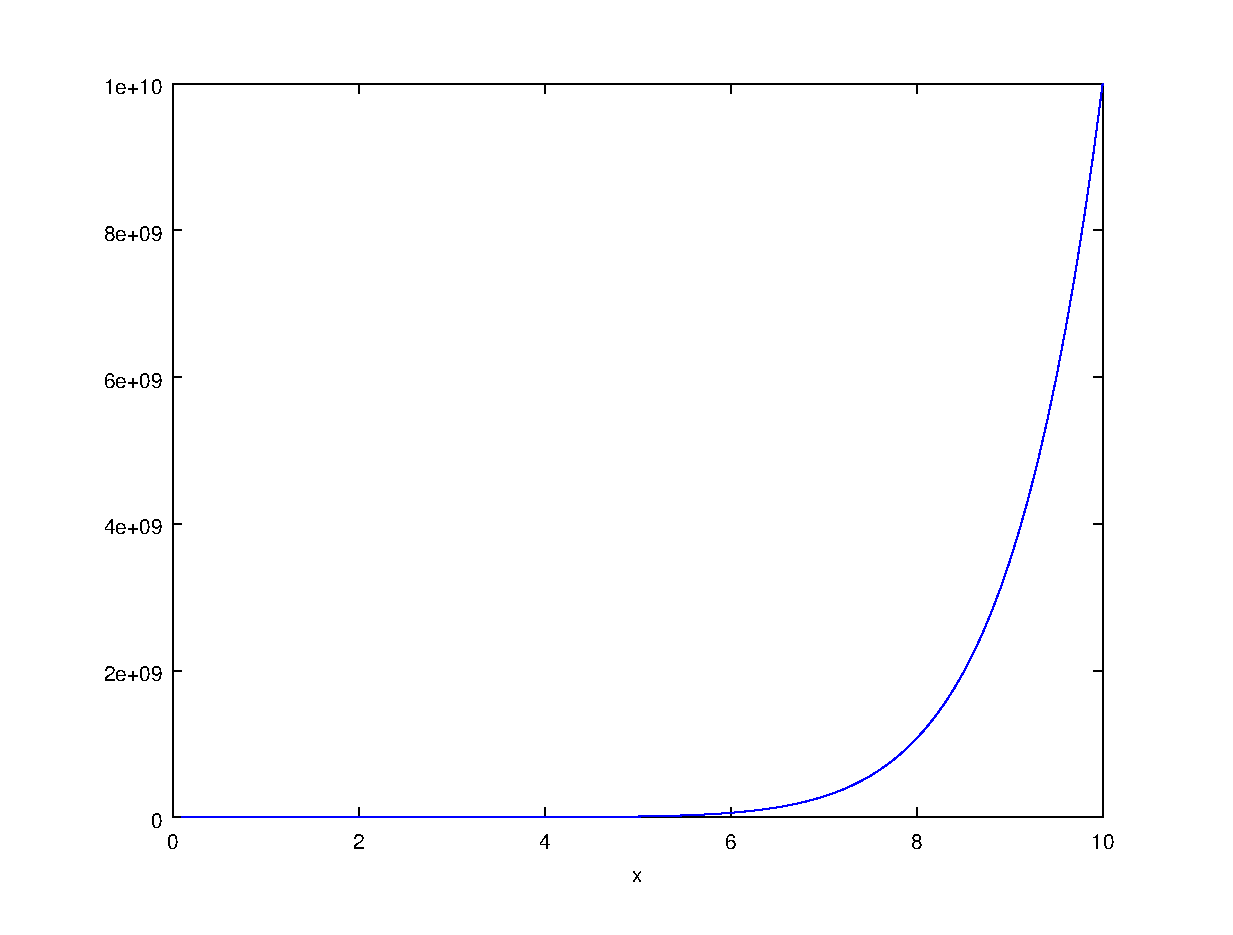
\includegraphics[width=0.8\textwidth]{1.eps}
\subsection{Let $z=ydx=x^2e^xdx$ and z(0)=0.}

\subsubsection{Find z using the numeric tools of MATLAB when $0 < x < 1.$} 
\begin{lstlisting}
	x = linspace(0,1,1001);
	y = x.**2.*exp(x);
	plot(x,y)
\end{lstlisting}

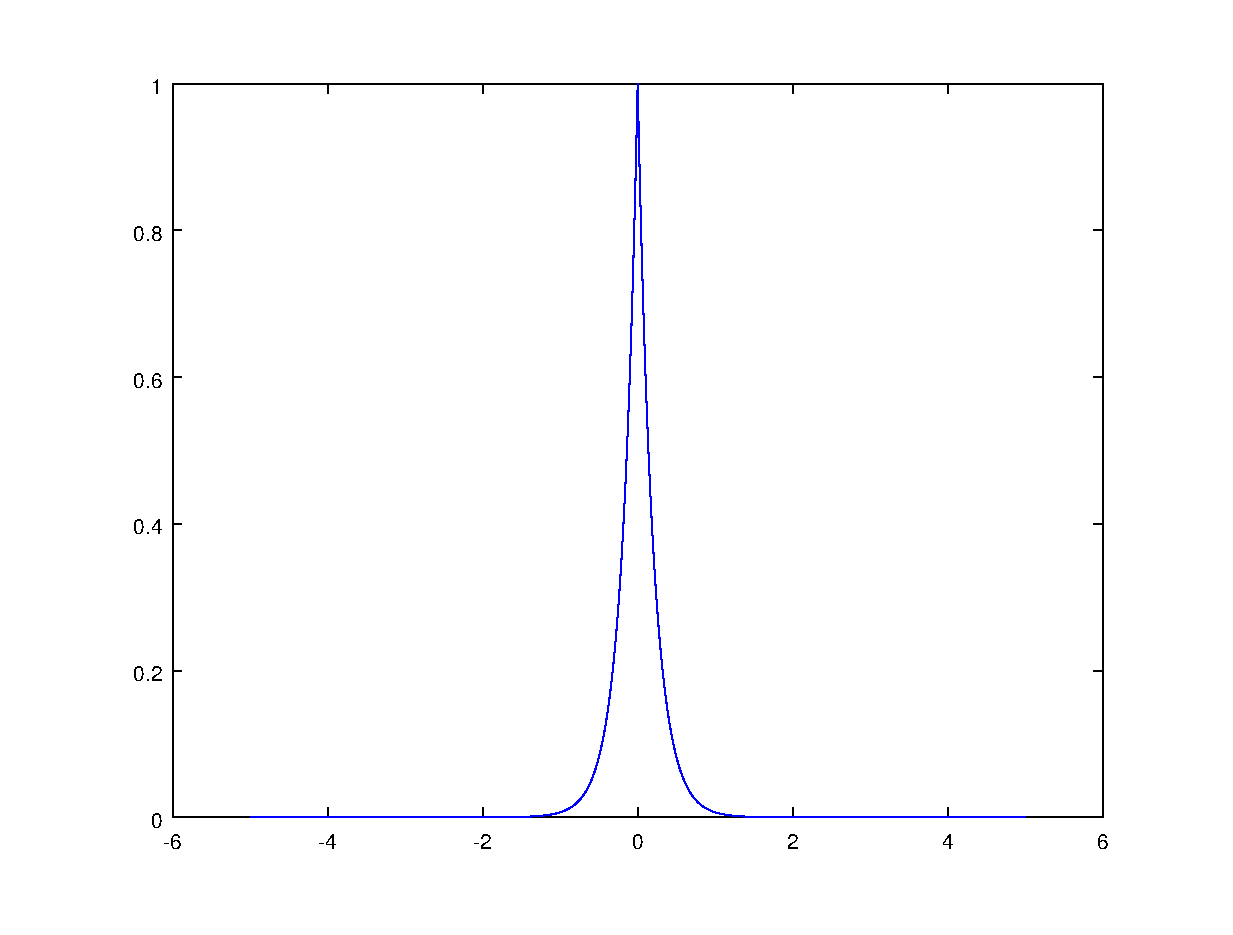
\includegraphics[width=0.8\textwidth]{2.eps}
\subsubsection{Plot y and z when $0 < x < 1$.}
\lstinputlisting{2.m}
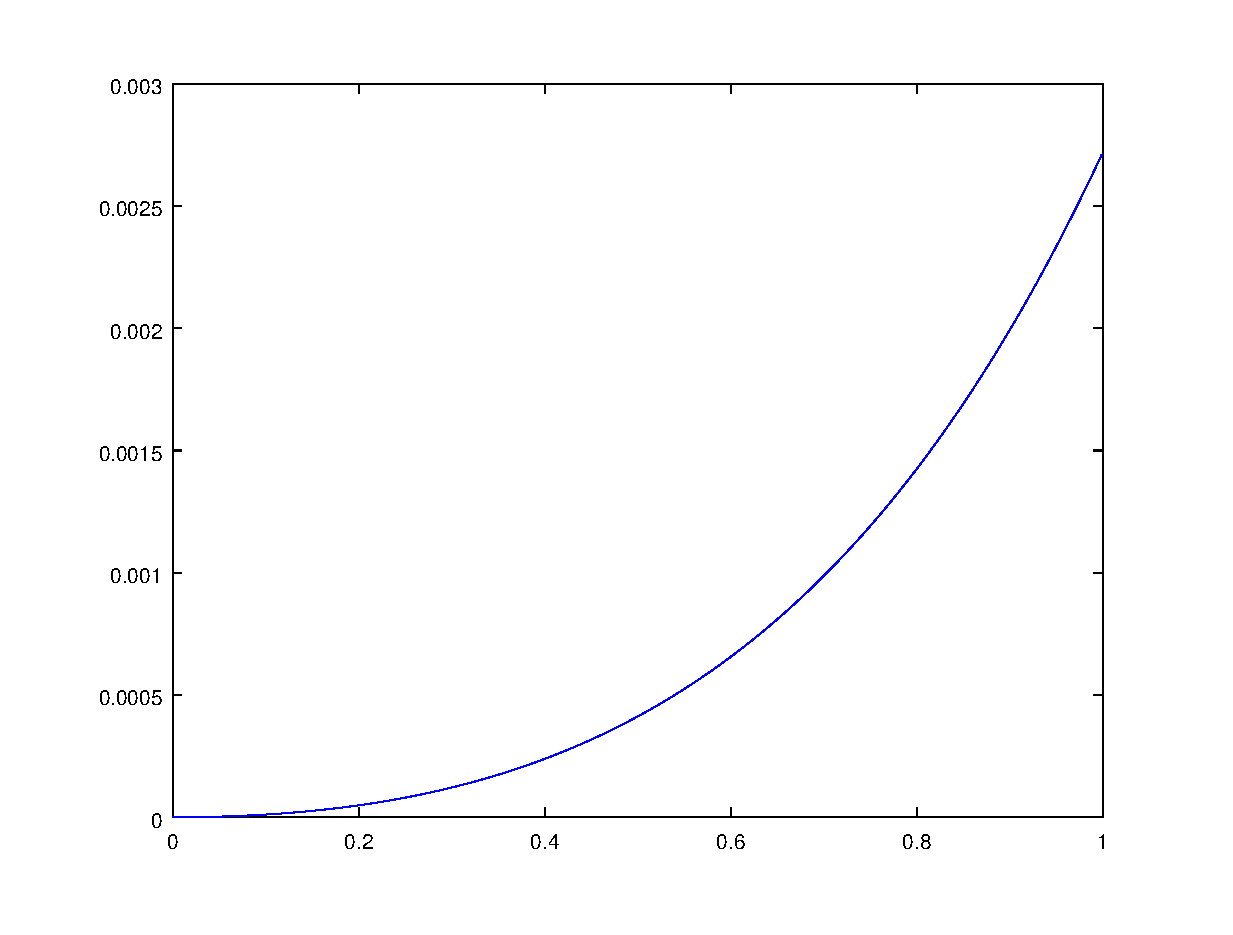
\includegraphics[width=0.8\textwidth]{2-2.eps}
\subsection{Let y = cos x, determine numerical derivative based on 101 points in one cycle and plot y’ and (-sinx).} 
\lstinputlisting{4.m}
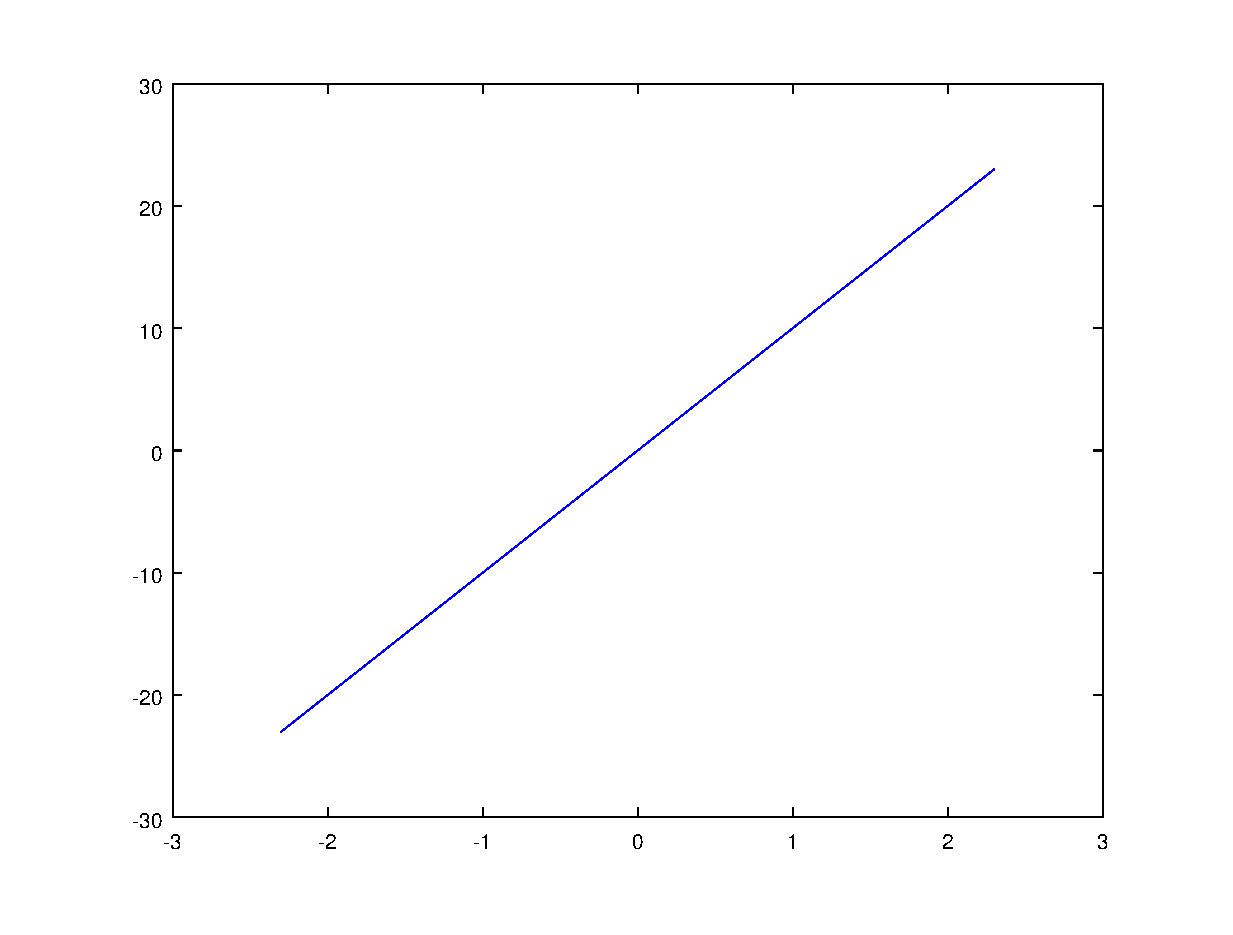
\includegraphics[width=0.8\textwidth]{4.eps}
\subsection{A test is performed on a mechanical part and the acceleration versus time is measured and shown as follows. Use MATLAB to determine and plot the velocity and displacement as a function of time.\\Remember that velocity = ∫ acceleration dt, and displacement = ∫ velocity dt.}

\includegraphics[width = \textwidth]{screenshot001.png}
\begin{lstlisting}
	t = [0:0.1:2];
	a=[0,9.05,16.37,22.22,26.81,30.33,32.93,34.76,35.95,36.59,
	36.79,36.62,36.14,35.43,34.52,33.47,32.30,
	31.06,29.75,28.42,27.07];
	v = 0.1 * cumsum(a);
	s = 0.1 * cumsum(v);
	plot(t,a, t,v, t,s)
\end{lstlisting}
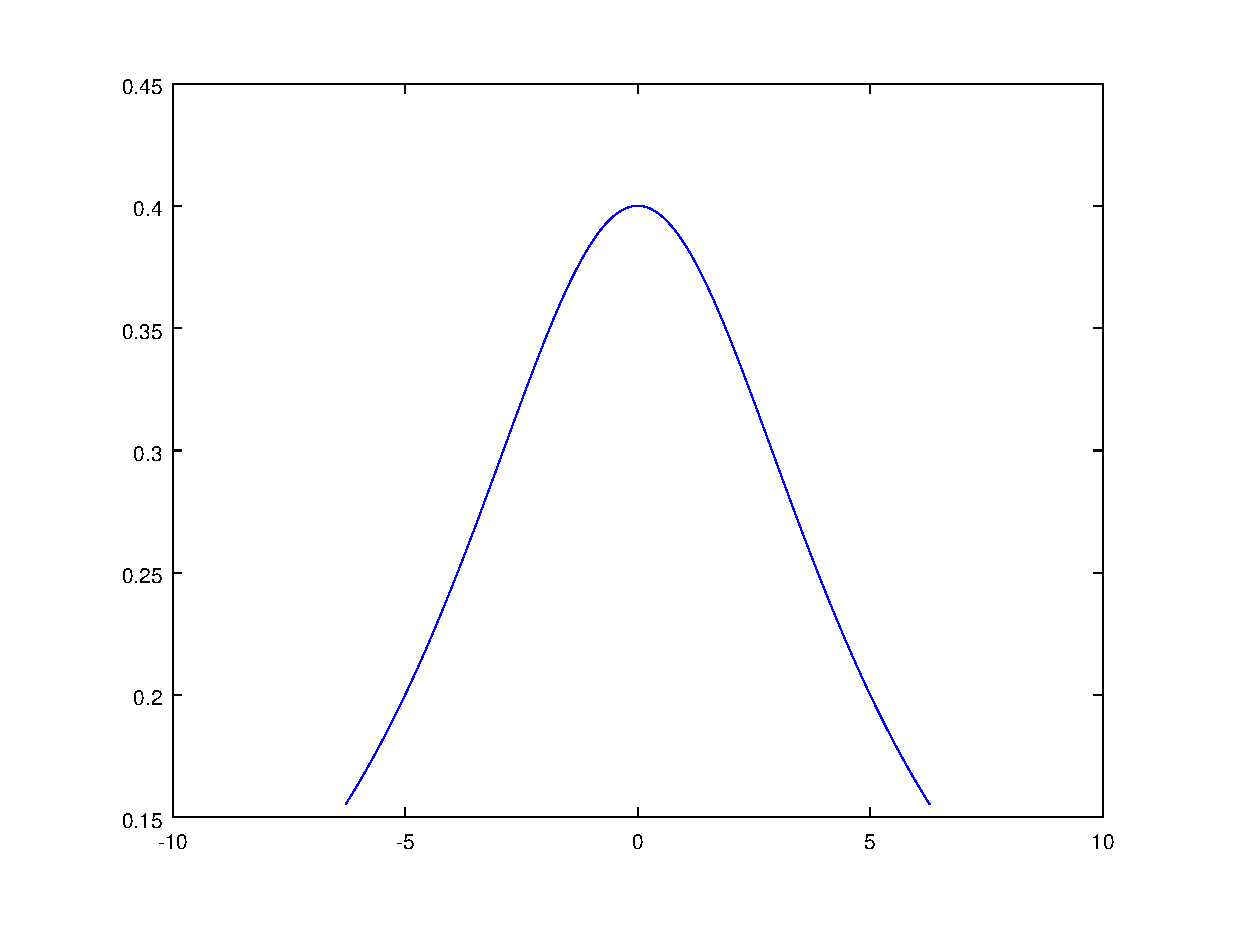
\includegraphics[width=0.8\textwidth]{3.eps}
\end{document}
